\chapter{\readyforreadingmod{A Framework for Building Verified Partial Evaluators}{maybe mentioning fusing compiler passes somewhere (but where?)}}\label{ch:rewriting}

\section{Introduction}\label{sec:rewriting:intro}

\begin{comment}
%\todonz{Drop intro}

Mechanized proof is gaining in importance for development of critical software infrastructure.
Oft-cited examples include the CompCert verified C compiler~\cite{Compcert} and the seL4 verified operating-system microkernel~\cite{seL4SOSP09}.
Here we have very flexible systems that are ready to adapt to varieties of workloads, be they C source programs for CompCert or application binaries for seL4.
For a verified operating system, such adaptation takes place at \emph{runtime}, when we launch the application.
However, some important bits of software infrastructure commonly do adaptation at \emph{compile time}, such that the fully general infrastructure software is not even installed in a deployed system.

Of course, compilers are a natural example of that pattern, as we would not expect CompCert itself to be installed on an embedded system whose application code was compiled with it.
The problem is that writing a compiler is rather labor-intensive, with its crafting of syntax-tree types for source, target, and intermediate languages, its fine-tuning of code for transformation passes that manipulate syntax trees explicitly, and so on.
An appealing alternative is \emph{partial evaluation}~\cite{PartialEvaluation}, which relies on reusable compiler facilities to specialize library code to parameters, with no need to write that library code in terms of syntax-tree manipulations.
Cutting-edge tools in this tradition even make it possible to use high-level functional languages to generate performance-competitive low-level code, as in Scala's Lightweight Modular Staging~\cite{LMS}.

It is natural to try to port this approach to construction of systems with mechanized proofs.
On one hand, the typed functional languages in popular proof assistants' logics make excellent hosts for flexible libraries, which can often be specialized through means as simple as partial application of curried functions.
Term-reduction systems built into the proof assistants can then generate the lean residual programs.
On the other hand, it is surprisingly difficult to realize the last sentence with good performance.
The challenge is that we are not just implementing algorithms; we also want a proof to be checked by a small proof checker, and there is tension in designing such a checker, as fancier reduction strategies grow the trusted code base.
It would seem like an abandonment of the spirit of proof assistants to bake in a reduction strategy per library, yet effective partial evaluation tends to be rather fine-tuned in this way.
Performance tuning matters when generated code is thousands of lines long.
\end{comment}

In this chapter, we present an approach to verified partial evaluation in proof assistants, which requires no changes to proof checkers.
To make the relevance concrete, we use the example of Fiat Cryptography~\cite{FiatCryptoSP19}, a Coq library that generates code for big-integer modular arithmetic at the heart of elliptic-curve-cryptography algorithms.
This domain-specific compiler has been adopted, for instance, in the Chrome Web browser, such that about half of all HTTPS connections from browsers are now initiated using code generated (with proof) by Fiat Cryptography.
However, Fiat Cryptography was only used successfully to build C code for the two most widely used curves (P-256 and Curve25519).
Our original method of partial evaluation timed out trying to compile code for the third most widely used curve (P-384).
Additionally, to achieve acceptable reduction performance, the library code had to be written manually in continuation-passing style.
\label{sec:rewriting:fiat-crypto-CPS}%
We will demonstrate a new Coq library that corrects both weaknesses, while maintaining the generality afforded by allowing rewrite rules to be mixed with partial evaluation.

\subsection{A Motivating Example}\label{sec:motivating-example}\label{sec:explain-ident.eagerly}\label{sec:explain-eval-rect}\label{sec:explain-'}

We are interested in partial-evaluation examples that mix higher-order functions, inductive datatypes, and arithmetic simplification.
For instance, consider the following Coq code.

\begin{minted}{coq}
Definition prefixSums (ls : list nat) : list nat :=
  let ls' := combine ls (seq 0 (length ls)) in
  let ls'' := map (λ p, fst p * snd p) ls' in
  let '(_, ls''') := fold_left (λ '(acc, ls''') n,
    let acc' := acc + n in (acc', acc' :: ls''')) ls'' (0, []) in
  ls'''.
\end{minted}
%\todo{Do we want to mention dlet?  We only get the specified output if we use dlet rather than let...}
% Adam's reaction: no, it will confuse readers too much to mention dlet this early.

This function first computes list \mintinline{coq}{ls'} that pairs each element of input list \mintinline{coq}{ls} with its position, so, for instance, list $[a; b; c]$ becomes $[(a, 0); (b, 1); (c, 2)]$.
Then we map over the list of pairs, multiplying the components at each position.
Finally, we traverse that list, building up a list of all prefix sums.

We would like to specialize this function to particular list lengths.
That is, we know in advance how many list elements we will pass in, but we do not know the values of those elements.
For a given length, we can construct a schematic list with one free variable per element.
For example, to specialize to length four, we can apply the function to list \mintinline{coq}{[a; b; c; d]}, and we expect this output:
\begin{minted}{coq}
let acc  := b + c * 2   in
let acc' := acc + d * 3 in
[acc'; acc; b; 0]
\end{minted}

Notice how subterm sharing via \mintinline{coq}{let}s is important.
As list length grows, we avoid quadratic blowup in term size through sharing.
Also notice how we simplified the first two multiplications with $a \cdot 0 = 0$ and $b \cdot 1 = b$ (each of which requires explicit proof in Coq), using other arithmetic identities to avoid introducing new variables for the first two prefix sums of \mintinline{coq}{ls''}, as they are themselves constants or variables, after simplification.

To set up our partial evaluator, we prove the algebraic laws that it should use for simplification, starting with basic arithmetic identities.
\begin{minted}{coq}
Lemma zero_plus : ∀ n, 0 + n = n.  Lemma times_zero : ∀ n, n * 0 = 0.
Lemma plus_zero : ∀ n, n + 0 = n.  Lemma times_one  : ∀ n, n * 1 = n.
\end{minted}

Next, we prove a law for each list-related function, connecting it to the primitive-recursion combinator for some inductive type (natural numbers or lists, as appropriate).
We use a special apostrophe marker to indicate a quantified variable that may only match with \emph{compile-time constants}.
We also use a further marker \mintinline{coq}{ident.eagerly} to ask the reducer to simplify a case of primitive recursion by complete traversal of the designated argument's constructor tree.
%\todo{Hey, it sure would be nice to generate all of these to-eliminator lemmas automatically, too!  Next step for the plugin?}
%\todo{Reply from Jason: This is actually quite tricky, and I want to claim that it is significantly beyond the scope of the rewriter.  If you have a constant which is already defined in terms of the eliminator, it's quite easy for me to write a tactic that makes the one-step unfolding lemma.  And it's also quite easy to throw \mintinline{coq}{ident.eagerly} in front.  However, if the constant is not already defined in terms of the eliminator constant, and is instead a fixpoint, then you need something that is basically as powerful as Lean's elaborator to figure out the right recursion principle.}
\begin{minted}{coq}
Lemma eval_map A B (f : A -> B) l
: map f l = ident.eagerly list_rect _ _ [] (λ x _ l', f x :: l') l.
Lemma eval_fold_left A B (f : A -> B -> A) l a
: fold_left f l a
  = ident.eagerly list_rect _ _ (λ a, a) (λ x _ r a, r (f a x)) l a.
Lemma eval_combine A B (la : list A) (lb : list B)
: combine la lb =
  list_rect _
    (λ _, [])
    (λ x _ r lb, list_case (λ _, _)
    [] (λ y ys, (x,y)::r ys) lb) la lb.
Lemma eval_length A (ls : list A)
: length ls = list_rect _ 0 (λ _ _ n, S n) ls.
\end{minted}
%\todo{Explain the Proper lemma and that eagerly is incompatible with do\_again.}
% I think would be too much too soon to talk about do\_again here.

With all the lemmas available, we can package them up into a rewriter, which triggers generation of a specialized rewrite procedure and its soundness proof.
Our Coq plugin introduces a new command \mintinline{coq}{Make} for building rewriters
\begin{minted}{coq}
Make rewriter := Rewriter For (zero_plus, plus_zero, times_zero, times_one,
  eval_map, eval_fold_left, do_again eval_length, do_again eval_combine,
  eval_rect nat, eval_rect list, eval_rect prod)
  (with delta) (with extra idents (seq)).
\end{minted}
Most inputs to \mintinline{coq}{Rewriter For} list quantified equalities to use for left-to-right rewriting.
However, we also use options \mintinline{coq}{do_again}, to request that some rules trigger an extra bottom-up pass after being used for rewriting; \mintinline{coq}{eval_rect}, to queue up eager evaluation of a call to a primitive-recursion combinator on a known recursive argument; \mintinline{coq}{with delta}, to request evaluation of all monomorphic operations on concrete inputs; and \mintinline{coq}{with extra idents}, to inform the engine of further permitted identifiers that do not appear directly in any of the rewrite rules.

Our plugin also provides new tactics like \mintinline{coq}{Rewrite_rhs_for}, which applies a rewriter to the right-hand side of an equality goal.
That last tactic is just what we need to synthesize a specialized \mintinline{coq}{prefixSums} for list length four, along with a proof of its equivalence to the original function.
\begin{minted}{coq}
Definition prefixSums4 :
 { f : nat → nat → nat → nat → list nat
 | ∀ a b c d, f a b c d = prefixSums [a; b; c; d] }
  := ltac:(eexists; Rewrite_rhs_for rewriter; reflexivity).
\end{minted}


\subsection{Concerns of Trusted-Code-Base Size}\label{sec:trusted-code-base-size}

Crafting a reduction strategy is challenging enough in a standalone tool.
A large part of the difficulty in a proof assistant is reducing in a way that leaves a proof trail that can be checked efficiently by a small kernel.
Most proof assistants present user-friendly surface tactic languages that generate proof traces in terms of more-elementary tactic steps.
The trusted proof checker only needs to know about the elementary steps, and there is pressure to be sure that these steps are indeed elementary, not requiring excessive amounts of kernel code.
However, hardcoding a new reduction strategy in the kernel can bring dramatic performance improvements.
Generating thousands of lines of code with partial evaluation would be intractable if we were outputting sequences of primitive rewrite steps justifying every little term manipulation, so we must take advantage of the time-honored feature of type-theoretic proof assistants that reductions included in the definitional equality need not be requested explicitly.
We discuss the performance issues in more detail in \nameref{sec:setoid-rewrite-bottlenecks} in \autoref{sec:setoid-rewrite-bottlenecks}.

Which kernel-level reductions \emph{does} Coq support today?
Currently, the trusted code base knows about four different kinds of reduction: left-to-right conversion, right-to-left conversion, a virtual machine (VM) written in C based on the OCaml compiler, and a compiler to native code.
Furthermore, the first two are parameterized on an arbitrary user-specified ordering of which constants to unfold when, in addition to internal heuristics about what to do when the user has not specified an unfolding order for given constants.
Recently, native support for 63-bit integers~\cite{coq-pr-int63} and IEEE 754-2008 binary64 floats~\cite{coq-pr-floats} have been added to the VM and native machines.
A recent pull request proposes adding support for native arrays~\cite{coq-pr-parray}.

% Not sure if we want to include the following. -Adam
%% Some users of Coq are concerned by this increase in the TCB.
%% Out of the 34\,000 lines of code in the Coq kernel (about 5\,000 of them comments), about 4\,250 lines are the native compiler\footnote{In files matching \texttt{kernel/*native*}.}, about 6\,650 additional lines are dedicated to the VM\footnote{In files matching \texttt{kernel/*vm*}, \texttt{kernel/*byte*}, \texttt{kernel/cemitcodes*}, \texttt{kernel/clambda*}, \texttt{kernel/csymtable*}, \texttt{kernel/vconv*}, and \texttt{kernel/genOpcodeFiles*}.}, and an additional 3\,100 lines are devoted to conversion and reduction\footnote{In \texttt{kernel/reduction*}, \texttt{kernel/cClosure*}, \texttt{kernel/primred*}, and \texttt{kernel/conv\_oracle*}.}.

To summarize, there has been quite a lot of ``complexity creep'' in the Coq trusted base, to support efficient reduction, and yet realistic partial evaluation has \emph{still} been rather challenging.
Even the additional three reduction mechanisms outside Coq's kernel (\texttt{cbn}, \texttt{simpl}, \texttt{cbv}) are not at first glance sufficient for verified partial evaluation.

%% Definition foo \defeq
%%      (Pipeline.BoundsPipeline
%%         true None [64; 128]
%%         ltac:(let r \defeq Reify (fun f g => mulmod (weight 51 1) (2^255) [(1,19)] 5 f g) in
%%               exact r)
%%                (Some (repeat (@None _) 5), ((Some (repeat (@None _) 5), tt)))
%%                ZRange.type.base.option.None).
%%
%% Time Compute foo.
%%
%% Definition bar \defeq
%%      (Pipeline.BoundsPipeline
%%         true None [64; 128]
%%         ltac:(let r \defeq Reify (fun f g => mulmod (weight 51 2) (2^255) [(1,19)] 10 f g) in
%%               exact r)
%%                (Some (repeat (@None _) 10), ((Some (repeat (@None _) 10), tt)))
%%                ZRange.type.base.option.None).
%%
%% Time Compute bar.

\subsection{Our Solution}\label{sec:our-solution}

\textcite{Aehlig} presented a very relevant solution to a related problem, using \emph{normalization by evaluation (NbE)}~\cite{NbE} to bootstrap reduction of open terms on top of full reduction, as built into a proof assistant.
However, it was simultaneously true that they expanded the proof-assistant trusted code base in ways specific to their technique, and that they did not report any experiments actually using the tool for partial evaluation (just traditional full reduction), potentially hiding performance-scaling challenges or other practical issues.
We have adapted their approach in a new Coq library embodying \textbf{the first partial-evaluation approach to satisfy the following criteria}.

\begin{itemize}
\item It integrates with a general-purpose, foundational proof assistant, \textbf{without growing the trusted base}.
\item For a wide variety of initial functional programs, it provides \textbf{fast} partial evaluation with reasonable memory use.
\item It allows reduction that \textbf{mixes} \emph{rules of the definitional equality} with \emph{equalities proven explicitly as theorems}.
\item It \textbf{preserves sharing} of common subterms.
\item It also allows \textbf{extraction of standalone partial evaluators}.
\end{itemize}

Our contributions include answers to a number of challenges that arise in scaling NbE-based partial evaluation in a proof assistant.
First, we rework the approach of \textcite{Aehlig} to function \emph{without extending a proof assistant's trusted code base}, which, among other challenges, requires us to prove termination of reduction and encode pattern matching explicitly (leading us to adopt the performance-tuned approach of \textcite{maranget2008compiling}).

Second, using partial evaluation to generate residual terms thousands of lines long raises \emph{new scaling challenges}:
\begin{itemize}
\item
  Output terms may contain so \emph{many nested variable binders} that we expect it to be performance-prohibitive to perform bookkeeping operations on first-order-encoded terms (e.g., with de Bruijn indices, as is done in \Rtac{} by \textcite{rtac}).
  For instance, while the reported performance experiments of \textcite{Aehlig} generate only closed terms with no binders, Fiat Cryptography may generate a single routine (e.g., multiplication for curve P-384) with nearly a thousand nested binders.
%\todo{Consider being more specific here about expected cost of first-order representation, maybe using some experiment.}
%  \todo{Note from Jason: We haven't actually checked that the bookkeeping is performance-prohibitive.  I suspect there will be a cost, but that if when we made fiat-crypto there was an existing system that used de Bruijn indices and did this, (along with built-in let-lifting, etc), I suspect we might have been a bit more sad, but not prohibitively more sad.  I think we should be much more tentative with this bullet point.}
\item
  Naïve representation of terms without proper \emph{sharing of common subterms} can lead to fatal term-size blow-up.
  Fiat Cryptography's arithmetic routines rely on significant sharing of this kind.
\item
  Unconditional rewrite rules are in general insufficient, and we need \emph{rules with side conditions}.
  For instance, in Fiat Cryptography, some rules for simplifying modular arithmetic depend on proofs that operations in subterms do not overflow.
\item
  However, it is also not reasonable to expect a general engine to discharge all side conditions on the spot.
  We need integration with \emph{abstract interpretation} that can analyze whole programs to support reduction.
\end{itemize}

Briefly, our respective solutions to these problems are the \emph{parametric higher-order abstract syntax (PHOAS)}~\cite{PhoasICFP08} term encoding, a \emph{let-lifting} transformation threaded throughout reduction, extension of rewrite rules with executable Boolean side conditions, and a design pattern that uses decorator function calls to include analysis results in a program.

Finally, we carry out the \emph{first large-scale performance-scaling evaluation} of partial evaluation in a proof assistant, covering all elliptic curves from the published Fiat Cryptography experiments, along with microbenchmarks.

This chapter proceeds through explanations of the trust stories behind our approach and earlier ones (\autoref{sec:trust}), the core structure of our engine (\autoref{sec:structure}), the additional scaling challenges we faced (\autoref{sec:scaling}), performance experiments (\autoref{sec:evaluation}), and related work (\autoref{sec:related}) and conclusions.
Our implementation is available on GitHub at \url{https://github.com/mit-plv/rewriter}.%
\footnote{%
  The version described in this dissertation is available under the tag \href{https://github.com/mit-plv/rewriter/tree/v0.0.1}{v0.0.1}.
}


\section{Trust, Reduction, and Rewriting}\label{sec:trust}

Since much of the narrative behind our design process depends on trade-offs between performance and trustworthiness, we start by reviewing the general situation in proof assistants.

Across a variety of proof assistants, simplification of functional programs is a workhorse operation.
Proof assistants like Coq that are based on type theory typically build in \emph{definitional equality} relations, identifying terms up to reductions like $\beta$-reduction and unfolding of named identifiers.
What looks like a single ``obvious'' step in an on-paper equational proof may require many of these reductions, so it is handy to have built-in support for checking a claimed reduction.
\autoref{subfig:change} diagrams how such steps work in a system like Coq, where the system implementation is divided between a trusted \emph{kernel}, for checking \emph{proof terms} in a minimal language, and additional untrusted support, like a \emph{tactic} engine evaluating a language of higher-level proof steps, in the process generating proof terms out of simpler building blocks.
It is standard to include a primitive proof step that validates any reduction compatible with the definitional equality, as the latter is decidable.
The figure shows a tactic that simplifies a goal using that facility.

In proof goals containing free variables, executing subterms can get stuck before reaching normal forms.
However, we can often achieve further simplification by using equational rules that we prove explicitly, rather than just relying on the rules built into the definitional equality and its decidable equivalence checker.
Coq's \texttt{autorewrite} tactic, as diagrammed in \autoref{subfig:autorewrite}, is a good example: it takes in a database of quantified equalities and applies them repeatedly to rewrite in a goal.
It is important that Coq's kernel does not trust the \texttt{autorewrite} tactic.
Instead, the tactic must output a proof term that, in some sense, is the moral equivalent of a line-by-line equational proof.
It can be challenging to keep these proof terms small enough, as naïve rewrite-by-rewrite versions repeatedly copy large parts of proof goals, justifying a rewrite like $C[e_1] = C[e_2]$ for some context $C$ given a proof of $e_1 = e_2$, with the full value of $C$ replicated in the proof term for that single rewrite.
Overcoming these challenges while retaining decidability of proof checking is tricky, since we may use \texttt{autorewrite} with rule sets that do not always lead to terminating reduction.
Coq includes more experimental alternatives like \texttt{rewrite\_strat}, which use bottom-up construction of multi-rewrite proofs, with sharing of common contexts.
Still, as \autoref{sec:evaluation} will show, these methods that generate substantial proof terms are at significant performance disadvantages.
We also experimented with the corresponding tactics in the Lean proof assistant, with similarly disappointing results (\autoref{sec:lean}).

\begin{figure} \centering
  \subfloat[Reduction via the definitional equality]{%
    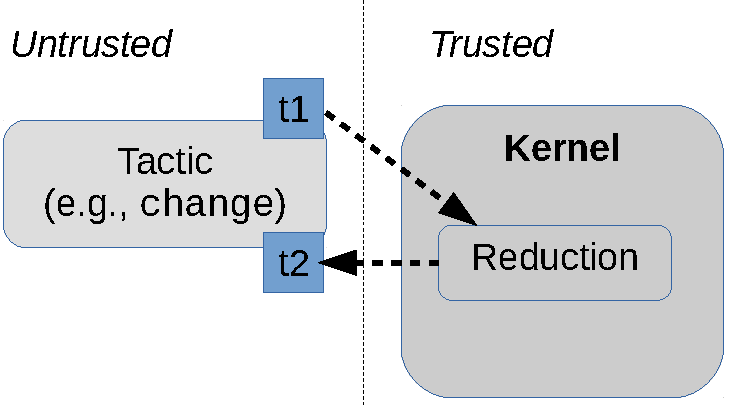
\includegraphics[width=0.48\textwidth]{rewriting/trust1}
    \label{subfig:change}} \hfill %\\
  \subfloat[Rewriting via proved rules]{%
    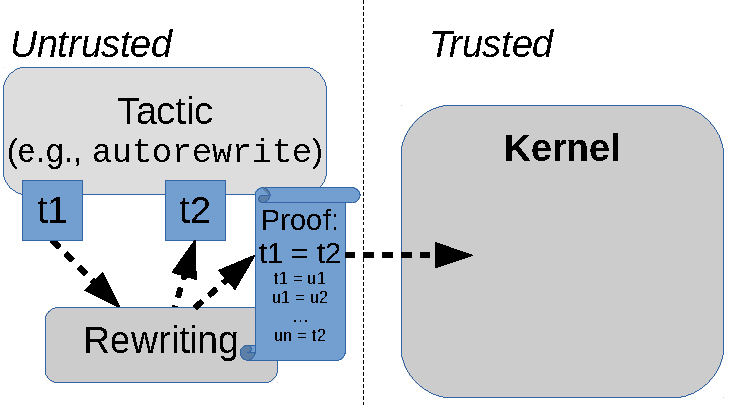
\includegraphics[width=0.48\textwidth]{rewriting/trust2}
    \label{subfig:autorewrite}} \\
  \subfloat[Approach of \textcite{Aehlig}]{%
    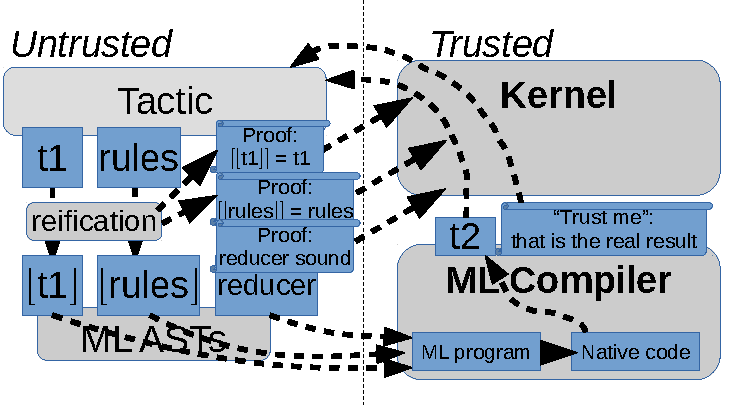
\includegraphics[width=0.48\textwidth]{rewriting/trust3}
    \label{subfig:aehlig}} \hfill %\\
  \subfloat[Our approach]{%
    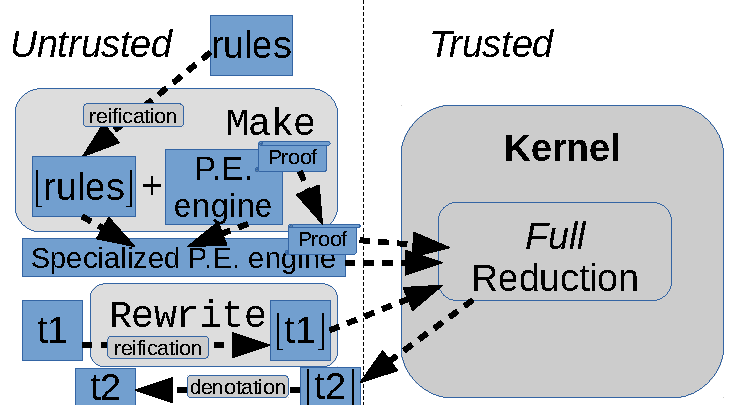
\includegraphics[width=0.48\textwidth]{rewriting/trust4}
    \label{subfig:perfect}}

  \caption{Different approaches to reduction and rewriting}
  \label{fig:trust}
\end{figure}

Now we summarize how \textcite{Aehlig} provide flexible and fast interleaving of standard $\lambda$-calculus reduction and use of proved equalities (the next section will go into more detail).
\autoref{subfig:aehlig} demonstrates a workflow based on \emph{a deep embedding of a core ML-like language}.
That is, within the logic of the proof assistant (Isabelle/HOL, in their case), a type of syntax trees for ML programs is defined, with an associated operational semantics.
The basic strategy is, for a particular set of rewrite rules and a particular term to simplify, to \emph{generate a (deeply embedded) ML program that, if it terminates, produces a syntax tree for the simplified term}.
Their tactic uses \emph{reification} to create ML versions of rule sets and terms.
They also wrote a reduction function in ML and proved it sound once and for all, against the ML operational semantics.
Combining that proof with proofs generated by reification, we conclude that an application of the reduction function to the reified rules and term is indeed an ML term that generates correct answers.
The tactic then ``throws the ML term over the wall,'' using a general code-generation framework for Isabelle/HOL~\cite{CodeGen}.
Trusted code compiles the ML code into the concrete syntax of a mainstream ML language, Standard ML in their case, and compiles it with an off-the-shelf compiler.
The output of that compiled program is then passed back over to the tactic, in terms of an axiomatic assertion that the ML semantics really yields that answer.

As \textcite{Aehlig} argue, their use of external compilation and evaluation of ML code adds no real complexity on top of that required by the proof assistant -- after all, the proof assistant itself must be compiled and executed somehow.
However, the perceived increase of trusted code base is not spurious:
it is one thing to trust that the toolchain and execution environment used by the proof assistant and the partial evaluator are well-behaved,
and another to rely on two descriptions of ML (one deeply embedded in the proof assistant and another implied by the compiler) to agree on every detail of the semantics.
Furthermore, there still is new trusted code to translate from the deeply embedded ML subset into the concrete syntax of the full-scale ML language.
% Aehlig et al. defined an ML language quite specialized to their use case, building in exactly the one algebraic datatype they need to represent NbE results, and it is unsatisfying to add such a specialized translator to the trusted base.
% However, we could imagine using a very general deep embedding of the proof assistant in itself, as with Template-Coq~\cite{TemplateCoq}.
% In that case, the expansion of the trusted code base would be even more worrying, to include an interpretation function from a complete syntactic embedding of the language within itself.
% Any inconsistency between the mechanized operational semantics (which would not be small, for a full-scale practical logic) and the actual implementation could break logical soundness.
The vast majority of proof-assistant developments today rely on no such embeddings with associated mechanized semantics, so need we really add one to a proof-checking kernel to support efficient partial evaluation?

Our answer, diagrammed in \autoref{subfig:perfect}, shows a different way.
We still reify terms and rules into a deeply embedded language.
However, \emph{the reduction engine is implemented directly in the logic}, rather than as a deeply embedded syntax tree of an ML program.
As a result, the kernel's own reduction engine is prepared to execute our reduction engine for us -- using an operation that would be included in a type-theoretic proof assistant in any case, with no special support for a language deep embedding.
We also stage the process for performance reasons.
First, the \mintinline{coq}{Make} command creates a rewriter out of a list of rewrite rules, by specializing a generic partial-evaluation engine, which has a generic proof that applies to any set of proved rewrite rules.
We perform partial evaluation on the specialized partial evaluator, using Coq's normal reduction mechanisms, under the theory that we can afford to pay performance costs at this stage because we only need to create new rewriters relatively infrequently.
Then individual rewritings involve reifying terms, asking the kernel to execute the specialized evaluator on them, and simplifying an application of an interpretation function to the result (this last step must be done using Coq's normal reduction, and it is the bottleneck for outputs with enormous numbers of nested binders as discussed in section \ref{sec:micro}).

We would like to emphasize that, while we prototyped our implementation in Coq in particular, the trade-off space that we navigate seems fundamental, so that it should be the case both that our approach can be adapted to other proof assistants and that this case study may inform proof-assistant design.
The general game here is to stock the trusted proof-checking kernel with as few primitive rules as we can get away with, while still providing enough flexibility and performance.
Every proof assistant we are aware of has a small functional language at its core, and we argue that is quite natural to include a primitive for efficient full reduction of programs.
Our empirical result is that such a primitive can form the basis for bootstrapping other kinds of efficient reduction, perhaps suggesting that a future Coq version could fruitfully shrink its kernel by eliminating other built-in reduction strategies.

\subsection{Our Approach in Nine Steps}\label{sec:nine-steps}

Here is a bit more detail on the steps that go into applying our Coq plugin, many of which we expand on in the following sections.
In order to build a precomputed rewriter with the \mintinline{coq}{Make} command, the following actions are performed:
\begin{enumerate}
\item
  The given lemma statements are scraped for which named functions and types the rewriter package will support.
\item
  Inductive types enumerating all available primitive types and functions are emitted.
\item
  Tactics generate all of the necessary definitions and prove all of the necessary lemmas for dealing with this particular set of inductive codes.
  Definitions include operations like Boolean equality on type codes and lemmas like ``all representable primitive types have decidable equality.''
\item
  The statements of rewrite rules are reified and soundness and syntactic-well-formedness lemmas are proven about each of them.
  Each instance of the former involves wrapping the user-provided proof with the right adapter to apply to the reified version.
\item
  The definitions needed to perform reification and rewriting and the lemmas needed to prove correctness are assembled into a single package that can be passed by name to the rewriting tactic.
\end{enumerate}

When we want to rewrite with a rewriter package in a goal, the following steps are performed:
\begin{enumerate}
\item
  We rearrange the goal into a single logical formula: all free-variable quantification in the proof context is replaced by changing the equality goal into an equality between two functions (taking the free variables as inputs).
  %\todo{Pedantic Note From Jason: it's not actually an equality between two functions, it's an \mintinline{coq}{equiv} between two functions where \mintinline{coq}{equiv} is a custom relation we define indexed over type codes that is equality up to function extensionality}
\item
  We reify the side of the goal we want to simplify, using the inductive codes in the specified package.  That side of the goal is then replaced with a call to a denotation function on the reified version.
\item
  We use a theorem stating that rewriting preserves denotations of well-formed terms to replace the denotation subterm with the denotation of the rewriter applied to the same reified term.
  We use Coq's built-in full reduction (\texttt{vm\_compute}) to reduce the application of the rewriter to the reified term.
\item
  Finally, we run \texttt{cbv} (a standard call-by-value reducer) to simplify away the invocation of the denotation function on the concrete syntax tree from rewriting.
  %\todo{Is it worth mentioning that we'd instead use \texttt{vm\_compute} if it supported whitelists (and also said whitelists were recorded in the casts)?}
\end{enumerate}


\section{The Structure of a Rewriter}\label{sec:structure}

We now simultaneously review the approach of \textcite{Aehlig} and introduce some notable differences in our own approach, noting similarities to the reflective rewriter of \textcite{rtac} where applicable.

First, let us describe the language of terms we support rewriting in.
Note that, while we support rewriting in full-scale Coq proofs, where the metalanguage is dependently typed, the object language of our rewriter is nearly simply typed, with limited support for calling polymorphic functions.
However, we still support identifiers whose definitions use dependent types, since our reducer does not need to look into definitions.
\begin{align*}
  e ::={}& \phantom{\mid} \texttt{App }e_1\texttt{ }e_2 \mid \texttt{Let }v \defeq e_1\texttt{ In }e_2 %\\
  %&
  \mid \texttt{Abs }(\lambda v.\,e) \mid \texttt{Var }v \mid \texttt{Ident }i
\end{align*}
The \texttt{Ident} case is for identifiers, which are described by an enumeration specific to a use of our library.
For example, the identifiers might be codes for $+$, $\cdot$, and literal constants.
We write $\llbracket e \rrbracket$ for a standard denotational semantics.

\subsection{Pattern-Matching Compilation and Evaluation}\label{sec:pattern-matching-compilation-and-evaluation}

\textcite{Aehlig} feed a specific set of user-provided rewrite rules to their engine by generating code for an ML function, which takes in deeply embedded term syntax (actually \emph{doubly} deeply embedded, within the syntax of the deeply embedded ML!) and uses ML pattern matching to decide which rule to apply at the top level.
Thus, they delegate efficient implementation of pattern matching to the underlying ML implementation.
As we instead build our rewriter in Coq's logic, we have no such option to defer to ML.
Indeed, Coq's logic only includes primitive pattern-matching constructs to match one constructor at a time.
%The frontend desugars nested pattern matching into trees of matches, but we do not have access to that desugaring within the language.
%It is arguably a good design decision to keep Coq working this way, since putting efficient nested pattern matching into the kernel would grow the trusted base substantially.

We could follow a naïve strategy of repeatedly matching each subterm against a pattern for every rewrite rule, as in the rewriter of \textcite{rtac}, but in that case we do a lot of duplicate work when rewrite rules use overlapping function symbols.
Instead, we adopted the approach of \textcite{maranget2008compiling}, who describes compilation of pattern matches in OCaml to decision trees that eliminate needless repeated work (for example, decomposing an expression into $x + y + z$ only once even if two different rules match on that pattern).
We have not yet implemented any of the optimizations described therein for finding \emph{minimal} decision trees.

There are three steps to turn a set of rewrite rules into a functional program that takes in an expression and reduces according to the rules.
The first step is pattern-matching compilation: we must compile the left-hand sides of the rewrite rules to a decision tree that describes how and in what order to decompose the expression, as well as describing which rewrite rules to try at which steps of decomposition.
Because the decision tree is merely a decomposition hint, we require no proofs about it to ensure soundness of our rewriter.
The second step is decision-tree evaluation, during which we decompose the expression as per the decision tree, selecting which rewrite rules to attempt.
The only correctness lemma needed for this stage is that any result it returns is equivalent to picking some rewrite rule and rewriting with it.
The third and final step is to actually rewrite with the chosen rule.
Here the correctness condition is that we must not change the semantics of the expression.
Said another way, any rewrite-rule replacement expression must match the semantics of the rewrite-rule pattern.

While pattern matching begins with comparing one pattern against one expression, Maranget's approach works with intermediate goals that check multiple patterns against multiple expressions.
A decision tree describes how to match a vector (or list) of patterns against a vector of expressions.
It is built from these constructors:
\begin{itemize}
  \item \texttt{TryLeaf k onfailure}: Try the $k^\text{th}$ rewrite rule; if it fails, keep going with \texttt{onfailure}.
  \item \texttt{Failure}: Abort; nothing left to try.
  \item \texttt{Switch icases app\_case default}:
    With the first element of the vector, match on its kind; if it is an identifier matching something in \texttt{icases}, which is a list of pairs of identifiers and decision trees, remove the first element of the vector and run that decision tree; if it is an application and \texttt{app\_case} is not \texttt{None}, try the \texttt{app\_case} decision tree, replacing the first element of each vector with the two elements of the function and the argument it is applied to; otherwise, do not modify the vectors and use the \texttt{default} decision tree.
  \item \texttt{Swap i cont}: Swap the first element of the vector with the $i^\texttt{th}$ element (0-indexed) and keep going with \texttt{cont}.
\end{itemize}

Consider the encoding of two simple example rewrite rules, where we follow Coq's \Ltac{} language in prefacing pattern variables with question marks.
\begin{align*}
  ?n + 0 & \to n %\\
  &
  \texttt{fst}_{\mathbb{Z},\mathbb{Z}}(?x, ?y) & \to x
\end{align*}
We embed them in an AST type for patterns, which largely follows our ASTs for expressions.
\begin{verbatim}
0. App (App (Ident +) Wildcard) (Ident (Literal 0))
1. App (Ident fst) (App (App (Ident pair) Wildcard) Wildcard)
\end{verbatim}
The decision tree produced is \label{sec:compiled-pattern}
\[\xymatrix@C+0.5pc@R-1pc{
  *++[o][F-]\txt{} \ar[d]_{\txt{App}} \\
  *++[o][F-]\txt{} \ar[r]^-{\txt{App}} \ar@/_1.5pc/[dr]_{\txt{\texttt{fst}}} & *++[o][F-]\txt{} \ar[r]^-{+} & *++[o][F-]\txt{Swap 0$\leftrightarrow$1} \ar[r] & *++[o][F-]\txt{} \ar[rr]^-{\txt{\texttt{Literal~0}}} && *++[o][F-]\txt{TryLeaf 0} \\
  & *++[o][F-]\txt{} \ar[r]_-{\txt{App}} & *++[o][F-]\txt{} \ar[r]_-{\txt{App}} & *++[o][F-]\txt{} \ar[rr]_-{\txt{\texttt{pair}}} && *++[o][F-]\txt{TryLeaf 1}
}\]
\noindent where every nonswap node implicitly has a ``default'' case arrow to \texttt{Failure} and circles represent \texttt{Switch} nodes.

We implement, in Coq's logic, an evaluator for these trees against terms.
Note that we use Coq's normal partial evaluation to turn our general decision-tree evaluator into a specialized matcher to get reasonable efficiency.
Although this partial evaluation of our partial evaluator is subject to the same performance challenges we highlighted in the introduction, it only has to be done once for each set of rewrite rules, and we are targeting cases where the time of per-goal reduction dominates this time of meta-compilation.

For our running example of two rules, specializing gives us this match expression.
\begin{minted}{coq}
match e with
| App f y => match f with
  | Ident fst => match y with
    | App (App (Ident pair) x) y => x | _ => e end
  | App (Ident +) x => match y with
    | Ident (Literal 0) => x | _ => e end | _ => e end | _ => e end.
\end{minted}

\subsection{Adding Higher-Order Features}\label{sec:thunk-eval-subst-term}

Fast rewriting at the top level of a term is the key ingredient for supporting customized algebraic simplification.
However, not only do we want to rewrite throughout the structure of a term, but we also want to integrate with simplification of higher-order terms, in a way where we can prove to Coq that our syntax-simplification function always terminates.
Normalization by evaluation (NbE)~\cite{NbE} is an elegant technique for adding the latter aspect, in a way where we avoid needing to implement our own $\lambda$-term reducer or prove it terminating.

To orient expectations: we would like to enable the following reduction
\begin{align*}
  (\lambda f\ x\ y.\, f\ x\ y)\ (+)\ z\ 0 & \leadsto z
\end{align*}
\noindent using the rewrite rule
\begin{align*}
  ?n + 0 & \to n
\end{align*}

\textcite{Aehlig} also use NbE, and we begin by reviewing its most classic variant, for performing full $\beta$-reduction in a simply typed term in a guaranteed-terminating way.
The simply typed $\lambda$-calculus syntax we use is:
\begin{align*}
  t & ::= t \to t ~|~ b
  & e & ::= \lambda v.\, e ~|~ e~e ~|~ v ~|~ c
\end{align*}
\noindent with $v$ for variables, $c$ for constants, and $b$ for base types.

We can now define normalization by evaluation.
First, we choose a ``semantic'' representation for each syntactic type, which serves as the result type of an intermediate interpreter.
\label{sec:NbE_t}
\begin{align*}
  \text{NbE}_t(t_1 \to t_2) & \defeq \text{NbE}_t(t_1) \to \text{NbE}_t(t_2) \\
  \text{NbE}_t(b) & \defeq \texttt{expr}(b)
\end{align*}
Function types are handled as in a simple denotational semantics, while base types receive the perhaps-counterintuitive treatment that the result of ``executing'' one is a syntactic expression of the same type.
We write $\texttt{expr}(b)$ for the metalanguage type of object-language syntax trees of type $b$, relying on a type family $\texttt{expr}$.

\begin{figure}%[b]
\begin{align*}
  \text{reify}_t & : \text{NbE}_t(t) \to \text{expr}(t) \\
  \text{reify}_{t_1 \to t_2}(f) & \defeq \lambda v.\,\text{reify}_{t_2}(f(\text{reflect}_{t_1}(v))) \\
  \text{reify}_{b}(f) & \defeq f \\ \noalign{\vskip7pt}
  \text{reflect}_t & : \text{expr}(t) \to \text{NbE}_t(t) \\
  \text{reflect}_{t_1\to t_2}(e) & \defeq \lambda x.\,\text{reflect}_{t_2}(e(\text{reify}_{t_1}(x)) \\
  \text{reflect}_{b}(e) & \defeq e \\ \noalign{\vskip7pt}
  \text{reduce} & : \text{expr}(t) \to \text{NbE}_t(t) \\
  \text{reduce}(\lambda v. \; e) & \defeq \lambda x. \; \text{reduce}([x/v]e) \\
  \text{reduce}(e_1~e_2) & \defeq \left(\text{reduce}(e_1)\right)(\text{reduce}(e_2)) \\
  \text{reduce}(x) & \defeq x \\
  \text{reduce}(c) & \defeq \text{reflect}(c) \\ \noalign{\vskip7pt}
  \text{NbE} & : \text{expr}(t) \to \text{expr}(t) \\
  \text{NbE}(e) & \defeq \text{reify}(\text{reduce}(e))
\end{align*}
\caption{\label{fig:nbe}Implementation of normalization by evaluation}
\end{figure}

Now the core of NbE, shown in \autoref{fig:nbe}, is a pair of dual functions reify and reflect, for converting back and forth between syntax and semantics of the object language, defined by primitive recursion on type syntax.
We split out analysis of term syntax in a separate function reduce, defined by primitive recursion on term syntax, when usually this functionality would be mixed in with reflect.
The reason for this choice will become clear when we extend NbE to handle our full problem domain.

% These definitions apply some of the usual corner-cutting that we see in on-paper descriptions of $\lambda$-term transformations.
We write $v$ for object-language variables and $x$ for metalanguage (Coq) variables, and we overload $\lambda$ notation using the metavariable kind to signal whether we are building a host $\lambda$ or a $\lambda$ syntax tree for the embedded language.
The crucial first clause for reduce replaces object-language variable $v$ with fresh metalanguage variable $x$, and then we are somehow tracking that all free variables in an argument to reduce must have been replaced with metalanguage variables by the time we reach them.
We reveal in \autoref{sec:PHOAS} the encoding decisions that make all the above legitimate, but first let us see how to integrate use of the rewriting operation from the previous section.
To fuse NbE with rewriting, we only modify the constant case of \texttt{reduce}.
First, we bind our specialized decision-tree engine under the name rewrite-head.
Recall that this function only tries to apply rewrite rules at the top level of its input.

In the constant case, we still reflect the constant, but underneath the binders introduced by full $\eta$-expansion, we perform one instance of rewriting.
In other words, we change this one function-definition clause:
\begin{align*}
  \text{reflect}_{b}(e) & \defeq \text{rewrite-head}(e)
\end{align*}

It is important to note that a constant of function type will be $\eta$-expanded only once for each syntactic occurrence in the starting term, though the expanded function is effectively a thunk, waiting to perform rewriting again each time it is called.
From first principles, it is not clear why such a strategy terminates on all possible input terms, though we work up to convincing Coq of that fact.

The details so far are essentially the same as in the approach of \textcite{Aehlig}.
Recall that their rewriter was implemented in a deeply embedded ML, while ours is implemented in Coq's logic, which enforces termination of all functions.
Aehlig et al. did not prove termination, which indeed does not hold for their rewriter in general, which works with untyped terms, not to mention the possibility of rule-specific ML functions that diverge themselves.
In contrast, we need to convince Coq up-front that our interleaved $\lambda$-term normalization and algebraic simplification always terminate.
Additionally, we need to prove that our rewriter preserves denotations of terms, which can easily devolve into tedious binder bookkeeping, depending on encoding.

The next section introduces the techniques we use to avoid explicit termination proof or binder bookkeeping, in the context of a more general analysis of scaling challenges.


\section{Scaling Challenges}\label{sec:scaling}

\textcite{Aehlig} only evaluated their implementation against closed programs.
What happens when we try to apply the approach to partial-evaluation problems that should generate thousands of lines of low-level code?

\subsection{Variable Environments Will Be Large}\label{sec:PHOAS}
We should think carefully about representation of ASTs, since many primitive operations on variables will run in the course of a single partial evaluation.
For instance, \textcite{Aehlig} reported a significant performance improvement changing variable nodes from using strings to using de Bruijn indices~\cite{debruijn1972}.
However, de Bruijn indices and other first-order representations remain painful to work with.
We often need to fix up indices in a term being substituted in a new context.
Even looking up a variable in an environment tends to incur linear time overhead, thanks to traversal of a list.
Perhaps we can do better with some kind of balanced-tree data structure, but there is a fundamental performance gap versus the arrays that can be used in imperative implementations.
Unfortunately, it is difficult to integrate arrays soundly in a logic.
Also, even ignoring performance overheads, tedious binder bookkeeping complicates proofs.

Our strategy is to use a variable encoding that pushes all first-order bookkeeping off on Coq's kernel, which is itself performance-tuned with some crucial pieces of imperative code.
Parametric higher-order abstract syntax (PHOAS)~\cite{PhoasICFP08}, which we introduced and described in \autoref{sec:binders:PHOAS}, is a dependently typed encoding of syntax where binders are managed by the enclosing type system.
It allows for relatively easy implementation and proof for NbE, so we adopted it for our framework.

Here is the actual inductive definition of term syntax for our object language, PHOAS-style.
The characteristic oddity is that the core syntax type \texttt{expr} is parameterized on a dependent type family for representing variables.
However, the final representation type \texttt{Expr} uses first-class polymorphism over choices of variable type, bootstrapping on the metalanguage's parametricity to ensure that a syntax tree is agnostic to variable type.
\begin{minted}{coq}
Inductive type := arrow (s d : type) | base (b : base_type).
Infix "→" := arrow.

Inductive expr (var : type -> Type) : type -> Type :=
| Var {t} (v : var t) : expr var t
| Abs {s d} (f : var s -> expr var d) : expr var (s → d)
| App {s d} (f : expr var (s → d)) (x : expr var s) : expr var d
| Const {t} (c : const t) : expr var t

Definition Expr (t : type) : Type := forall var, expr var t.
\end{minted}

A good example of encoding adequacy is assigning a simple denotational semantics.
First, a simple recursive function assigns meanings to types.
\begin{minted}{coq}
Fixpoint denoteT (t : type) : Type
  := match t with
     | arrow s d => denoteT s -> denoteT d
     | base b    => denote_base_type b
     end.
\end{minted}

Next we see the convenience of being able to \emph{use} an expression by choosing how it should represent variables.
Specifically, it is natural to choose \emph{the type-denotation function itself} as the variable representation.
Especially note how this choice makes rigorous the convention we followed in the prior section (e.g., in the suspicious function-abstraction clause of function reduce), where a recursive function enforces that values have always been substituted for variables early enough.
\begin{minted}{coq}
Fixpoint denoteE {t} (e : expr denoteT t) : denoteT t
  := match e with
     | Var v     => v
     | Abs f     => λ x, denoteE (f x)
     | App f x   => (denoteE f) (denoteE x)
     | Ident c   => denoteI c
     end.
Definition DenoteE {t} (E : Expr t) : denoteT t
  := denoteE (E denoteT).
\end{minted}

It is now easy to follow the same script in making our rewriting-enabled NbE fully formal.
Note especially the first clause of \texttt{reduce}, where we avoid variable substitution precisely because we have chosen to represent variables with normalized semantic values.
The subtlety there is that base-type semantic values are themselves expression syntax trees, which depend on a nested choice of variable representation, which we retain as a parameter throughout these recursive functions.
The final definition $\lambda$-quantifies over that choice.
\begin{minted}{coq}
Fixpoint nbeT var (t : type) : Type
  := match t with
     | arrow s d => nbeT var s -> nbeT var d
     | base b    => expr var b
     end.

Fixpoint reify {var t} : nbeT var t -> expr var t
  := match t with
     | arrow s d => λ f, Abs (λ x, reify (f (reflect (Var x))))
     | base b    => λ e, e
     end
with reflect {var t} : expr var t -> nbeT var t
  := match t with
     | arrow s d => λ e, λ x, reflect (App e (reify x))
     | base b    => rewrite_head
     end.

Fixpoint reduce {var t}
  (e : expr (nbeT var) t) : nbeT var t
  := match e with
     | Abs e     => λ x, reduce (e (Var x))
     | App e1 e2 => (reduce e1) (reduce e2)
     | Var x     => x
     | Ident c   => reflect (Ident c)
     end.

Definition Rewrite {t} (E : Expr t) : Expr t
  := λ var, reify (reduce (E (nbeT var t))).
\end{minted}

One subtlety hidden above in implicit arguments is in the final clause of \texttt{reduce}, where the two applications of the \texttt{Ident} constructor use different variable representations.
With all those details hashed out, we can prove a pleasingly simple correctness theorem, with a lemma for each main definition, with inductive structure mirroring recursive structure of the definition, also appealing to correctness of last section's pattern-compilation operations.
$$\forall t, E : \mintinline{coq}{Expr t}. \; \llbracket \mintinline{coq}{Rewrite}(E) \rrbracket = \llbracket E \rrbracket$$

Even before getting to the correctness theorem, we needed to convince Coq that the function terminates.
While for \textcite{Aehlig}, a termination proof would have been a whole separate enterprise, it turns out that PHOAS and NbE line up so well that Coq accepts the above code with no additional termination proof.
As a result, the Coq kernel is ready to run our \mintinline{coq}{Rewrite} procedure during checking.

To understand how we now apply the soundness theorem in a tactic, it is important to note how the Coq kernel builds in reduction strategies.
These strategies have, to an extent, been tuned to work well to show equivalence between a simple denotational-semantics application and the semantic value it produces.
In contrast, it is rather difficult to code up one reduction strategy that works well for all partial-evaluation tasks.
Therefore, we should restrict ourselves to (1) running full reduction in the style of functional-language interpreters and (2) running normal reduction on ``known-good'' goals like correctness of evaluation of a denotational semantics on a concrete input.

Operationally, then, we apply our tactic in a goal containing a term $e$ that we want to partially evaluate.
In standard proof-by-reflection style, we \emph{reify} $e$ into some $E$ where $\llbracket E \rrbracket = e$, replacing $e$ accordingly, asking Coq's kernel to validate the equivalence via standard reduction.
Now we use the \mintinline{coq}{Rewrite} correctness theorem to replace $\llbracket E \rrbracket$ with $\llbracket \mintinline{coq}{Rewrite}(E) \rrbracket$.
Next we may ask the Coq kernel to simplify $\mintinline{coq}{Rewrite}(E)$ by \emph{full reduction via compilation to native code}, since we carefully designed $\mintinline{coq}{Rewrite}(E)$ and its dependencies to produce closed syntax trees, so that reduction will not get stuck pattern-matching on free variables.
Finally, where $E'$ is the result of that reduction, we simplify $\llbracket E' \rrbracket$ with standard reduction, producing a normal-looking Coq term.

%% The payoffs from fully satisfying Coq's type checker are:
%% \begin{enumerate}
%% \item We know that this procedure always terminates, and Coq's kernel is therefore willing to run the procedure for us implicitly during proof checking.  In a sense, we have bootstrapped this reduction strategy into the conversion rule of the type theory.
%% \item In that setting, all bookkeeping about variable binding and environments is handled by the kernel, whose implementation in OCaml allows certain efficient implementation strategies not available to us in the logic.
%% \end{enumerate}

\subsection{Subterm Sharing Is Crucial}\label{sec:under-lets}

For some large-scale partial-evaluation problems, it is important to represent output programs with sharing of common subterms.
Redundantly inlining shared subterms can lead to exponential increase in space requirements.
Consider the Fiat Cryptography~\cite{FiatCryptoSP19} example of generating a 64-bit implementation of field arithmetic for the P-256 elliptic curve.
The library has been converted manually to continuation-passing style, allowing proper generation of \mintinline{coq}{let} binders, whose variables are often mentioned multiple times.
We ran their code generator (actually just a subset of its functionality, but optimized by us a bit further, as explained in \autoref{sec:macro}) on the P-256 example and found it took about 15 seconds to finish.
Then we modified reduction to inline \mintinline{coq}{let} binders instead of preserving them, at which point the reduction job terminated with an out-of-memory error, on a machine with 64 GB of RAM.
(The successful run uses under 2 GB.)

We see a tension here between performance and niceness of library implementation.
In our original implementation of Fiat Cryptography, we found it necessary to CPS-convert our code to coax Coq into adequate reduction performance.
Then all of our correctness theorems were complicated by reasoning about continuations.
It feels like a slippery slope on the path to implementing a domain-specific compiler, rather than taking advantage of the pleasing simplicity of partial evaluation on natural functional programs.
Our reduction engine takes shared-subterm preservation seriously while applying to libraries in direct style.

Our approach is \mintinline{coq}{let}-lifting: we lift \mintinline{coq}{let}s to top level, so that applications of functions to \mintinline{coq}{let}s are available for rewriting.
For example, we can perform the rewriting
\begin{align*}
  \texttt{map}\ (\lambda x.\, y+x)\ (\letin[{z:=e}{[0;1;2;z;z+1]}]) \\
  \leadsto \; \letin[{z:=e}{[y;y+1;y+2;y+z;y+(z+1)]}]
\end{align*}
using the rules
\begin{align*}
  \texttt{map}\ {?f}\ [] & \to []
  &
  \texttt{map}\ {?f}\ ({?x} :: {?xs}) & \to f\ x :: \texttt{map}\ f\ xs
  & {?n} + 0 & \to n %\\
\end{align*}

Our approach is to define a telescope-style type family called \mintinline{coq}{UnderLets}:
\begin{minted}{coq}
Inductive UnderLets {var} (T : Type) :=
| Base (v : T)
| UnderLet {A}(e : @expr var A)(f : var A -> UnderLets T).
\end{minted}
A value of type \mintinline{coq}{UnderLets T} is a series of \texttt{let} binders (where each expression \mintinline{coq}{e} may mention earlier-bound variables) ending in a value of type \mintinline{coq}{T}.
It is easy to build various ``smart constructors'' working with this type, for instance to construct a function application by lifting the \texttt{let}s of both function and argument to a common top level.

Such constructors are used to implement an NbE strategy that outputs \mintinline{coq}{UnderLets} telescopes.
Recall that the NbE type interpretation mapped base types to expression syntax trees.
We now parameterize that type interpretation by a Boolean declaring whether we want to introduce telescopes.

\begin{minted}{coq}
Fixpoint nbeT' {var} (with_lets : bool) (t : type) :=
  match t with
  | base t
    => if with_lets then @UnderLets var (@expr var t) else @expr var t
  | arrow s d => nbeT' false s -> nbeT' true d
  end.
Definition nbeT := nbeT' false.
Definition nbeT_with_lets := nbeT' true.
\end{minted}

%%  - Here are some examples:
%%    - `value Z := UnderLets (expr Z)`
%%    - `value (Z -> Z) := expr Z -> UnderLets (expr Z)`
%%    - `value (Z -> Z -> Z) := expr Z -> expr Z -> UnderLets (expr Z)`
%%    - `value ((Z -> Z) -> Z) := (expr Z -> UnderLets (expr Z)) -> UnderLets (expr Z)`

There are cases where naïve preservation of \texttt{let} binders blocks later rewrites from triggering and leads to suboptimal performance, so we include some heuristics.
For instance, when the expression being bound is a constant, we always inline.
When the expression being bound is a series of list ``cons'' operations, we introduce a name for each individual list element, since such a list might be traversed multiple times in different ways.

\subsection{Rules Need Side Conditions}\label{sec:side-conditions}

Many useful algebraic simplifications require side conditions.
One simple case is supporting \emph{nonlinear} patterns, where a pattern variable appears multiple times.
We can encode nonlinearity on top of linear patterns via side conditions.
\begin{align*}
  {?n_1} + {?m} - {?n_2} & \to m\text{\ \ if\ \ }n_1 = n_2
\end{align*}

The trouble is how to support predictable solving of side conditions during partial evaluation, where we may be rewriting in open terms.
We decided to sidestep this problem by allowing side conditions only as executable Boolean functions, to be applied only to variables that are confirmed as \emph{compile-time constants}, unlike \textcite{rtac} who support general unification variables.
We added a variant of pattern variable that only matches constants.
Semantically, this variable style has no additional meaning, and in fact we implement it as a special identity function that should be called in the right places within Coq lemma statements.
Rather, use of this identity function triggers the right behavior in our tactic code that reifies lemma statements.
We introduce a notation where a prefixed apostrophe signals a call to the ``constants only'' function.

Our reification inspects the hypotheses of lemma statements, using type classes to find decidable realizations of the predicates that are used, synthesizing one Boolean expression of our deeply embedded term language, standing for a decision procedure for the hypotheses.
The \mintinline{coq}{Make} command fails if any such expression contains pattern variables not marked as constants.
Therefore, matching of rules can safely run side conditions, knowing that Coq's full-reduction engine can determine their truth efficiently.

\subsection{Side Conditions Need Abstract Interpretation}\label{sec:abs-int}

With our limitation that side conditions are decided by executable Boolean procedures, we cannot yet handle directly some of the rewrites needed for realistic partial evaluation.
For instance, Fiat Cryptography reduces high-level functional to low-level code that only uses integer types available on the target hardware.
The starting library code works with arbitrary-precision integers, while the generated low-level code should be careful to avoid unintended integer overflow.
As a result, the setup may be too naïve for our running example rule ${?n} + 0 \to n$.
When we get to reducing fixed-precision-integer terms, we must be legalistic:
\begin{align*}
  \texttt{add\_with\_carry}_{64}({?n}, 0) & \to (0, n)\text{\ \ if\ \ }0 \le n < 2^{64}
\end{align*}

We developed a design pattern to handle this kind of rule.

First, we introduce a family of functions $\texttt{clip}_{l,u}$, each of which forces its integer argument to respect lower bound $l$ and upper bound $u$.
Partial evaluation is proved with respect to unknown realizations of these functions, only requiring that $\texttt{clip}_{l, u}(n) = n$ when $l \leq n < u$.
Now, before we begin partial evaluation, we can run a verified abstract interpreter to find conservative bounds for each program variable.
When bounds $l$ and $u$ are found for variable $x$, it is sound to replace $x$ with $\texttt{clip}_{l,u}(x)$.
Therefore, at the end of this phase, we assume all variable occurrences have been rewritten in this manner to record their proved bounds.

Second, we proceed with our example rule refactored:
\begin{align*}
  \texttt{add\_with\_carry}_{64}(\texttt{clip}_{\texttt{'}{?l},\texttt{'}{?u}}({?n}), 0) & \to (0, \texttt{clip}_{l,u}(n)) %\\
  %&
  \text{\ \ if\ \ }u < 2^{64}
\end{align*}
If the abstract interpreter did its job, then all lower and upper bounds are constants, and we can execute side conditions straightforwardly during pattern matching.

\subsection{Limitations and Preprocessing}\label{sec:implementation-and-usage}

%\todo{It's not clear to Jason what in this section belongs here, and what isn't interesting (yet?) to readers}
%\todo{I (Jason) have no idea what the story for this section should be}
%\todo{Insofar as text is actually kept in this section, make sure any duplication between here and the out-of-paper appendix is deliberate}
%\todo{If this section is moved or removed, be sure to restructure \autoref{sec:code-from-implementation-and-usage} accordingly}

We now note some details of the rewriting framework that were previously glossed over, which are useful for using the code or implementing something similar, but which do not add fundamental capabilities to the approach.
Although the rewriting framework does not support dependently typed constants, we can automatically preprocess uses of eliminators like \mintinline{coq}{nat_rect} and \mintinline{coq}{list_rect} into nondependent versions.
The tactic that does this preprocessing is extensible via \Ltac{}'s reassignment feature.
Since pattern-matching compilation mixed with NbE requires knowing how many arguments a constant can be applied to, internally we must use a version of the recursion principle whose type arguments do not contain arrows; current preprocessing can handle recursion principles with either no arrows or one arrow in the motive.

Recall from \autoref{sec:explain-eval-rect} that \mintinline{coq}{eval_rect} is a definition provided by our framework for eagerly evaluating recursion associated with certain types.
It functions by triggering typeclass resolution for the lemmas reducing the recursion principle associated to the given type.
We provide instances for \texttt{nat}, \texttt{prod}, \texttt{list}, \texttt{option}, and \texttt{bool}.
Users may add more instances if they desire.

Recall again from \autoref{sec:explain-ident.eagerly} that we use \mintinline{coq}{ident.eagerly} to ask the reducer to simplify a case of primitive recursion by complete traversal of the designated argument's constructor tree.
Our current version only allows a limited, hard-coded set of eliminators with \mintinline{coq}{ident.eagerly} (\texttt{nat\_rect} on return types with either zero or one arrows, \texttt{list\_rect} on return types with either zero or one arrows, and \texttt{List.nth\_default}), but nothing in principle prevents automatic generation of the necessary code.

Note that \mintinline{coq}{Let_In} is the constant we use for writing \letin{} expressions that do not reduce under $\zeta$ (Coq's reduction rule for \mintinline{coq}{let}-inlining).
Throughout most of this chapter, anywhere that \letin{} appears, we have actually used \mintinline{coq}{Let_In} in the code.
It would alternatively be possible to extend the reification preprocessor to automatically convert \letin{} to \mintinline{coq}{Let_In}, but this strategy may cause problems when converting the interpretation of the reified term with the prereified term, as Coq's conversion does not allow fine-tuning of when to inline or unfold \mintinline{coq}{let}s.

\section{Evaluation}\label{sec:evaluation}

Our implementation, available on GitHub at \url{https://github.com/mit-plv/rewriter} with a roadmap in \autoref{sec:CodeSupplement-more}, includes a mix of Coq code for the proved core of rewriting, tactic code for setting up proper use of that core, and OCaml plugin code for the manipulations beyond the current capabilities of the tactic language.
We report here on experiments to isolate performance benefits for rewriting under binders and reducing higher-order structure.

\subsection{Microbenchmarks}\label{sec:micro}

\def\NoBindersSubfloatNval{3}%
\def\NoBindersSubfloatXRow{\thisrowno{0}*(2^(\nval+1)-1)}%

We start with microbenchmarks focusing attention on particular aspects of reduction and rewriting, with \autoref{sec:additionalMicro} going into more detail.

\bgroup
\interlinepenalty 10000
\subsubsection{Rewriting Without Binders}\label{sec:micro:Plus0Tree}

\begin{wrapfigure}[7]{r}{0pt}
{\small $\begin{aligned}
\text{iter}_m(v) & = v + \underbrace{0 + 0 + \cdots + 0}_m \\
\text{tree}_{0,m}(v) &= \text{iter}_m(v + v) \\
\text{tree}_{n+1,m}(v) &= \text{iter}_m(\text{tree}_{n,m}(v) + \text{tree}_{n,m}(v))
\end{aligned}$}%
\caption{\label{fig:micro:Plus0Tree:code}Expressions computing initial code}
\end{wrapfigure}
Consider the code defined by the expression $\text{tree}_{n,m}(v)$ in \autoref{fig:micro:Plus0Tree:code}.
%\todo{make sure the figure spacing is okay}
%RSolve[{t[0]==m, t[n]==2*t[n-1] + m},t[n],n]
%t[n]=m(2^{n+1}-1)
We want to remove all of the${}+0$s.
There are $\Theta(m \cdot 2^n)$ such rewriting locations.
We can start from this expression directly, in which case reification alone takes as much time as Coq's \texttt{rewrite}.
As the reification method was not especially optimized, and there exist fast reification methods~\cite{reification-by-parametricity}, we instead start from a call to a recursive function that generates such an expression.
\label{sec:reif-not-optimized}%

\egroup

\begin{figure}[btp]
  \newsavebox{\NestedBindersSubfloat}%
  \sbox{\NestedBindersSubfloat}{%
    \adjustbox{valign=t}{\resizebox{0.4\textwidth}{!}{\beginTikzpictureStamped[only marks]{
      \einput{rewriting/perf-UnderLetsPlus0-cbv;rewrite-strat(bottomup).txt}
      \einput{rewriting/perf-UnderLetsPlus0-cbv;rewrite-strat(topdown).txt}
      \einput{rewriting/perf-UnderLetsPlus0-cbv;setoid-rewrite.txt}
      \einput{rewriting/perf-UnderLetsPlus0-Rewrite-for.txt}
      \einput{rewriting/perf-UnderLetsPlus0-rewriting.txt}
    }
      \pgfplotsset{every axis legend/.append style={
          at={(0.5,-0.2)},
          anchor=north}}
      \begin{axis}[xlabel=\# of let binders,ylabel=time (s),ymax=65]
        \addplot[mark=o,color=red] table{rewriting/perf-UnderLetsPlus0-cbv;rewrite-strat(bottomup).txt};
        \addplot[mark=triangle,color=red] table{rewriting/perf-UnderLetsPlus0-cbv;rewrite-strat(topdown).txt};
        \addplot[mark=square,color=red] table{rewriting/perf-UnderLetsPlus0-cbv;setoid-rewrite.txt};
        \addplot[mark=+,color=blue] table{rewriting/perf-UnderLetsPlus0-Rewrite-for.txt};
        \addplot[mark=x,color=ForestGreen] table{rewriting/perf-UnderLetsPlus0-rewriting.txt};
        \legend{rewrite\_strat bottomup,rewrite\_strat topdown,setoid\_rewrite,{Our approach including reification, cbv, etc.},Our approach (only rewriting)}
      \end{axis}
    \end{tikzpicture}}}}%
  \newsavebox{\BindersAndRecursiveFunctionsSubfloat}%
  \sbox{\BindersAndRecursiveFunctionsSubfloat}{%
    \adjustbox{valign=t}{\resizebox{0.4\textwidth}{!}{\beginTikzpictureStamped[only marks]{
        \einput{rewriting/perf-LiftLetsMap-rewrite-strat(bottomup,bottomup).txt}
        \einput{rewriting/perf-LiftLetsMap-rewrite-strat(topdown,bottomup).txt}
        \einput{rewriting/perf-LiftLetsMap-setoid-rewrite.txt}
        \einput{rewriting/perf-LiftLetsMap-Rewrite-for.txt}
        \einput{rewriting/perf-LiftLetsMap-rewriting.txt}
        \einput{rewriting/perf-LiftLetsMap-cps+vm-compute.txt}
    }
      \pgfplotsset{every axis legend/.append style={
          at={(0.5,-0.2)},
          anchor=north}}
      \begin{axis}[xlabel=$n\cdot m$,ylabel=time (s),scaled x ticks=false,ymax=27]
        \addplot[mark=o,color=red] table{rewriting/perf-LiftLetsMap-rewrite-strat(bottomup,bottomup).txt};
        \addplot[mark=triangle,color=red] table{rewriting/perf-LiftLetsMap-rewrite-strat(topdown,bottomup).txt};
        \addplot[mark=square,color=red] table{rewriting/perf-LiftLetsMap-setoid-rewrite.txt};
        \addplot[mark=+,color=blue] table{rewriting/perf-LiftLetsMap-Rewrite-for.txt};
        \addplot[mark=x,color=ForestGreen] table{rewriting/perf-LiftLetsMap-rewriting.txt};
        \addplot[mark=*,color=purple] table{rewriting/perf-LiftLetsMap-cps+vm-compute.txt};
        \legend{rewrite\_strat bottomup,rewrite\_strat topdown,repeat setoid\_rewrite,{Our approach including reification, cbv, etc.},Our approach (only rewriting),cps+vm\_compute}
      \end{axis}
    \end{tikzpicture}}}}%
  \newsavebox{\NoBindersSubfloat}%
  \sbox{\NoBindersSubfloat}{%
    \edef\nval{\NoBindersSubfloatNval}%
    \adjustbox{valign=t}{\resizebox{0.4\textwidth}{!}{\beginTikzpictureStamped[only marks]{
        \einput{rewriting/perf-Plus0Tree-only-n-\nval-cbv;rewrite-strat(bottomup).txt}
        \einput{rewriting/perf-Plus0Tree-only-n-\nval-cbv;setoid-rewrite.txt}
        \einput{rewriting/perf-Plus0Tree-only-n-\nval-cbv;rewrite-strat(topdown).txt}
        \einput{rewriting/perf-Plus0Tree-only-n-\nval-cbv;rewrite!.txt}
        \einput{rewriting/perf-Plus0Tree-only-n-\nval-Rewrite-for.txt}
        \einput{rewriting/perf-Plus0Tree-only-n-\nval-rewriting.txt}
        \nval
    }
      \pgfplotsset{every axis legend/.append style={
          at={(0.5,-0.2)},
          anchor=north}}
      % since n = 1, we have 2^n=twice as many rewrite locations as the value on the x axis, so we need to double things
      %,xticklabel={\pgfkeys{/pgf/fpu}\pgfmathparse{2^\nval*\tick}$\mathsf{\pgfmathprintnumber{\pgfmathresult}}$}
      \begin{axis}[xlabel=\# of rewrite locations,scaled x ticks=false,ylabel=time (s),ymax=7]% ymax=10]
        \addplot[mark=square,color=red] table[x expr={\NoBindersSubfloatXRow}]{rewriting/perf-Plus0Tree-only-n-\nval-cbv;rewrite-strat(bottomup).txt};
        \addplot[mark=*,color=red] table[x expr={\NoBindersSubfloatXRow}]{rewriting/perf-Plus0Tree-only-n-\nval-cbv;setoid-rewrite.txt};
        \addplot[mark=triangle,color=red] table[x expr={\NoBindersSubfloatXRow}]{rewriting/perf-Plus0Tree-only-n-\nval-cbv;rewrite-strat(topdown).txt};
        \addplot[mark=o,color=red] table[x expr={\NoBindersSubfloatXRow}]{rewriting/perf-Plus0Tree-only-n-\nval-cbv;rewrite!.txt};
        \addplot[mark=+,color=blue] table[x expr={\NoBindersSubfloatXRow}]{rewriting/perf-Plus0Tree-only-n-\nval-Rewrite-for.txt};
        \addplot[mark=x,color=ForestGreen] table[x expr={\NoBindersSubfloatXRow}]{rewriting/perf-Plus0Tree-only-n-\nval-rewriting.txt};
        \legend{rewrite\_strat bottomup,setoid\_rewrite,rewrite\_strat topdown,rewrite!,{Our approach including reification, cbv, etc.},Our approach (only rewriting)}
      \end{axis}
    \end{tikzpicture}}}}%
  \newsavebox{\FiatCryptoSubfloat}%
  \sbox{\FiatCryptoSubfloat}{%
    \adjustbox{valign=t}{\resizebox{0.4\textwidth}{!}{\beginTikzpictureStamped[only marks]{
      \einput{rewriting/perf-new-vm-over-old-vm.txt.md5}
      \einput{rewriting/perf-old-vm-over-old-vm.txt.md5}
      \einput{rewriting/perf-new-extraction-over-old-vm.txt.md5}
    }
      \pgfplotsset{every axis legend/.append style={
          at={(0.5,-0.2)},
          anchor=north}}
      \begin{axis}[xlabel=prime,ylabel=slowdown factor over old approach,xmode=log, ymode=log,log basis x={2}]
        \addplot[mark=+] table{rewriting/perf-new-vm-over-old-vm.txt};
        \addplot[mark=o] table{rewriting/perf-old-vm-over-old-vm.txt};
        \addplot[mark=*] table{rewriting/perf-new-extraction-over-old-vm.txt};
        \legend{Our approach w/ Coq's VM,Old approach (handwritten-CPS+VM),Our approach w/ extracted OCaml}
      \end{axis}
    \end{tikzpicture}}}}%
  \newcommand{\vphantomSubfloatOne}{\vphantom{\usebox{\NestedBindersSubfloat}}\vphantom{\usebox{\NoBindersSubfloat}}}%
  \newcommand{\vphantomSubfloatTwo}{\vphantom{\usebox{\BindersAndRecursiveFunctionsSubfloat}}\vphantom{\usebox{\FiatCryptoSubfloat}}}%
  \subfloat[No binders]{\usebox{\NoBindersSubfloat}\vphantomSubfloatOne\label{fig:timing-Plus0Tree}}%
  \quad
  \subfloat[Nested binders]{\usebox{\NestedBindersSubfloat}\vphantomSubfloatOne\label{fig:timing-UnderLetsPlus0}}%
  \quad
  \subfloat[Binders and recursive functions]{\usebox{\BindersAndRecursiveFunctionsSubfloat}\vphantomSubfloatTwo\label{fig:timing-LiftLetsMap}}%
  \quad
  \subfloat[Fiat Cryptography]{\usebox{\FiatCryptoSubfloat}\vphantomSubfloatTwo\label{fig:scaling}}

  \caption{Timing of different partial-evaluation implementations}\label{fig:multi-timing}
\end{figure}

%RSolve[{t[0]==m, t[n]==2*t[n-1] + m},t[n],n]
%t[n]=m(2^{n+1}-1)
\Vref{fig:timing-Plus0Tree} shows the results for $n = \NoBindersSubfloatNval$ as we scale $m$.
The comparison points are Coq's \texttt{rewrite!}, \texttt{setoid\_rewrite}, and \texttt{rewrite\_strat}.
The first two perform one rewrite at a time, taking minimal advantage of commonalities across them and thus generating quite large, redundant proof terms.
The third makes top-down or bottom-up passes with combined generation of proof terms.
For our own approach, we list both the total time and the time taken for core execution of a verified rewrite engine, without counting reification (converting goals to ASTs) or its inverse (interpreting results back to normal-looking goals).

The comparison here is very favorable for our approach so long as $m > 2$.
The competing tactics spike upward toward timeouts at just around a thousand rewrite locations, while our engine is still under two seconds for examples with tens of thousands of rewrite locations.
When $m < 2$, Coq's \texttt{rewrite!} tactic does a little bit better than our engine, corresponding roughly to the overhead incurred by our term representation (which, for example, stores the types at every application node) when most of the term is in fact unchanged by rewriting.
See \autoref{sec:additionalPlots:Plus0Tree} for more detailed plots.

\subsubsection{Rewriting Under Binders}\label{sec:micro:UnderLetsPlus0}

\begin{wrapfigure}[5]{r}{0pt}
{\small $\begin{aligned}
  & \letin[{v_1 := v_0 + v_0 + 0}{}] \\ \noalign{\vskip-7pt}
  & \vdots \\ \noalign{\vskip-3pt}
  & \letin[{v_n := v_{n-1} + v_{n-1} + 0}{}] \\
  & v_n + v_n + 0
\end{aligned}$}%
%  & \letin[{v_2 := v_1 + v_1 + 0}{}] \\
\caption{\label{fig:micro:UnderLetsPlus0:code}Initial code}
\end{wrapfigure}

Consider now the code in \autoref{fig:micro:UnderLetsPlus0:code}, which is a version of the code above where redundant expressions are shared via \mintinline{coq}{let} bindings.

\Vref{fig:timing-UnderLetsPlus0} shows the results.
The comparison here is again very favorable for our approach.
The competing tactics spike upward toward timeouts at just a few hundred generated binders, while our engine is only taking about 10 seconds for examples with 5,000 nested binders.

\subsubsection{Performance Bottlenecks of Proof-Producing Rewriting}\label{sec:micro:setoid-rewrite-bottlenecks-lite}\label{sec:setoid-rewrite-bottlenecks}

Although we have made our comparison against the built-in tactics \mintinline{coq}{setoid_rewrite} and \mintinline{coq}{rewrite_strat}, by analyzing the performance in detail, we can argue that these performance bottlenecks are likely to hold for any proof assistant designed like Coq.
Detailed debugging reveals five performance bottlenecks in the existing rewriting tactics.
(This section goes into detail that readers not interested in proof-assistant minutiae may want to skip, turning ahead to \nameref{sec:micro:LiftLetsMap} \vpageref{sec:micro:LiftLetsMap}.)

\paragraph{Bad performance scaling in sizes of existential-variable contexts}

We found that even when there are no occurrences fully matching the rule, \mintinline{coq}{setoid_rewrite} can still be \emph{cubic} in the number of binders (or, more accurately, quadratic in the number of binders with an additional multiplicative linear factor of the number of head-symbol matches).
Rewriting without any successful matches takes nearly as much time as \mintinline{coq}{setoid_rewrite} in this microbenchmark; by the time we are looking at goals with 400 binders, the difference is less than 5\%.

We posit that this overhead comes from \mintinline{coq}{setoid_rewrite} looking for head-symbol matches and then creating evars (existential variables) to instantiate the arguments of the lemmas for each head-symbol-match location; hence even if there are no matches of the rule as a whole, there may still be head-symbol matches.
Since Coq uses a locally nameless representation~\cite{Engineering2008Aydemir} for its terms, evar contexts are necessarily represented as \emph{named} contexts.
Representing a substitution between named contexts takes linear space, even when the substitution is trivial, and hence each evar incurs overhead linear in the number of binders above it.
Furthermore, fresh-name generation in Coq is quadratic in the size of the context, and since evar-context creation uses fresh-name generation, the additional multiplicative factor likely comes from fresh-name generation.
(%
Note, though, that this pattern suggests that the true performance is quartic rather than merely cubic.
However, doing a linear regression on a $\log$-$\log$ of the data suggests that the performance is genuinely cubic rather than quartic.%
)
See \coqissue{12524} for more details.

Note that this overhead is inherent to the use of a locally nameless term representation.
To fix it, Coq would likely have to represent identity evar contexts using a compact representation, which is only naturally available for de Bruijn representations.
Any rewriting system that uses unification variables with a locally nameless (or named) context will incur at least quadratic overhead on this benchmark.

Note that \mintinline{coq}{rewrite_strat} uses exactly the same rewriting engine as \mintinline{coq}{setoid_rewrite}, just with a different strategy.
We found that \mintinline{coq}{setoid_rewrite} and \mintinline{coq}{rewrite_strat} have identical performance when there are no matches and generate identical proof terms when there are matches.
Hence we can conclude that the difference in performance between \mintinline{coq}{rewrite_strat} and \mintinline{coq}{setoid_rewrite} is entirely due to an increased number of failed rewrite attempts.

\paragraph{Proof-term size}

Setting aside the performance bottleneck in constructing the matches in the first place, we can ask the question: how much cost is associated to the proof terms?
One way to ask this question in Coq is to see how long it takes to run \mintinline{coq}{Qed}.
While \mintinline{coq}{Qed} time is asymptotically better, it is still quadratic in the number of binders.
This outcome is unsurprising, because the proof-term size is quadratic in the number of binders.
On this microbenchmark, we found that \mintinline{coq}{Qed} time hits one second at about 250 binders, and using the best-fit quadratic line suggests that it would hit 10 seconds at about 800 binders and 100 seconds at about 2\,500 binders.
While this may be reasonable for the microbenchmarks, which only contain as many rewrite occurrences as there are binders, it would become unwieldy to try to build and typecheck such a proof with a rule for every primitive reduction step, which would be required if we want to avoid manually CPS-converting the code in Fiat Cryptography.

The quadratic factor in the proof term comes because we repeat subterms of the goal linearly in the number of rewrites.
For example, if we want to rewrite \mintinline{coq}{f (f x)} into \mintinline{coq}{g (g x)} by the equation \mintinline{coq}{∀ x, f x = g x}, then we will first rewrite \mintinline{coq}{f x} into \mintinline{coq}{g x}, and then rewrite \mintinline{coq}{f (g x)} into \mintinline{coq}{g (g x)}.
Note that \mintinline{coq}{g x} occurs three times (and will continue to occur in every subsequent step).

\paragraph{Poor subterm sharing}

How easy is it to share subterms and create a linearly sized proof?
While it is relatively straightforward to share subterms using \mintinline{coq}{let} binders when the rewrite locations are not under any binders, it is not at all obvious how to share subterms when the terms occur under different binders.
Hence any rewriting algorithm that does not find a way to share subterms across different contexts will incur a quadratic factor in proof-building and proof-checking time, and we expect this factor will be significant enough to make applications to projects as large as Fiat Crypto infeasible.

\paragraph{Overhead from the \mintinline{coq}{let} typing rule}

Suppose we had a proof-producing rewriting algorithm that shared subterms even under binders.
Would it be enough?
It turns out that even when the proof size is linear in the number of binders, the cost to typecheck it in Coq is still quadratic!
The reason is that when checking that \texttt{f : T} in a context \mintinline{coq}{x := v}, to check that \mintinline{coq}{let x := v in f} has type \texttt{T} (assuming that \mintinline{coq}{x} does not occur in \texttt{T}), Coq will substitute \mintinline{coq}{v} for \mintinline{coq}{x} in \texttt{T}.
So if a proof term has $n$ \mintinline{coq}{let} binders (e.g., used for sharing subterms), Coq will perform $n$ substitutions on the type of the proof term, even if none of the \mintinline{coq}{let} binders are used.
If the number of \mintinline{coq}{let} binders is linear in the size of the type, there is quadratic overhead in proof-checking time, even when the proof-term size is linear.

We performed a microbenchmark on a rewriting goal with no binders (because there is an obvious algorithm for sharing subterms in that case) and found that the proof-checking time reached about one second at about 2\,000 binders and reached 10 seconds at about 7\,000 binders.
While these results might seem good enough for Fiat Cryptography, we expect that there are hundreds of thousands of primitive reduction/rewriting steps even when there are only a few hundred binders in the output term, and we would need \mintinline{coq}{let} binders for each of them.
Furthermore, we expect that getting such an algorithm correct would be quite tricky.

Fixing this quadratic bottleneck would, as far as we can tell, require deep changes in how Coq is implemented; it would either require reworking all of Coq to operate on some efficient representation of delayed substitutions paired with unsubstituted terms, or else it would require changing the typing rules of the type theory itself to remove this substitution from the typing rule for \mintinline{coq}{let}.
Note that there is a similar issue that crops up for function application and abstraction.

\paragraph{Inherent advantages of reflection}

Finally, even if this quadratic bottleneck were fixed, \textcite{Aehlig} reported a $10\times$--$100\times$ speed-up over the \emph{simp} tactic in Isabelle, which performs all of the intermediate rewriting steps via the kernel API.
Their results suggest that even if all of the superlinear bottlenecks were fixed---no small undertaking---rewriting and partial evaluation via reflection might still be orders of magnitude faster than any proof-term-generating tactic.

\subsubsection{Binders and Recursive Functions}\label{sec:micro:LiftLetsMap}

\begin{wrapfigure}[10]{r}{0pt}
{\small %\allowdisplaybreaks
$\begin{aligned}
  \text{map\_dbl}(\ell) & \defeq \begin{cases} [] & \text{if }\ell = [] \\
      \letin[{y := h + h}{}] & \text{if }\ell = h::t \\
      y :: \text{map\_dbl}(t) &
      \end{cases} \\
  \text{make}(n, m, v) & \defeq \begin{cases} [\underbrace{v, \ldots, v}_n] & \text{if }m = 0 \\
      \text{map\_dbl}(\text{make}(n, m-1, v)) & \text{if }m > 0
      \end{cases} \\
  \text{example}_{n, m} & \defeq \forall v,\ \text{make}(n, m, v) = []
\end{aligned}$}%
\caption{\label{fig:micro:LiftLetsMap:code}Initial code for binders and recursive functions}
\end{wrapfigure}

The next experiment uses the code in \autoref{fig:micro:LiftLetsMap:code}.
%Note that the ${}=[]$ at the end is just a dummy placeholder to allow us to check reduction and rewriting of this term.
Note that the \letin{} binding blocks further reduction of map\_dbl when we iterate it $m$ times in make, and so we need to take care to preserve sharing when reducing here.

\Vref{fig:timing-LiftLetsMap} compares performance between our approach, \texttt{repeat setoid\_rewrite}, and two variants of \texttt{rewrite\_strat}.
Additionally, we consider another option, which was adopted by Fiat Cryptography at a larger scale: rewrite our functions to improve reduction behavior.
Specifically, both functions are rewritten in continuation-passing style, which makes them harder to read and reason about but allows standard VM-based reduction to achieve good performance.
The figure shows that \texttt{rewrite\_strat} variants are essentially unusable for this example, with \texttt{setoid\_rewrite} performing only marginally better, while our approach applied to the original, more readable definitions loses ground steadily to VM-based reduction on CPS'd code.
On the largest terms ($n \cdot m > 20,000$), the gap is 6s vs.\ 0.1s of compilation time, which should often be acceptable in return for simplified coding and proofs, plus the ability to mix proved rewrite rules with built-in reductions.
Note that about 99\% of the difference between the full time of our method and just the rewriting is spent in the final \texttt{cbv} at the end, used to denote our output term from reified syntax.
We blame this performance on the unfortunate fact that reduction in Coq is quadratic in the number of nested binders present; see \coqbug{11151}.
%traded for simplified coding and proofs, plus the ability to mix proved rewrite rules with built-in reductions.
See \autoref{sec:LiftLetsMap-more} for more on this microbenchmark.

%\bgroup
%\interlinepenalty 10000
\subsubsection{Full Reduction}\label{sec:micro:Eratosthenes}

\begin{figure}%[16]{r}{0pt}
  %\resizebox{0.4\textwidth}{!}{%
    \beginTikzpictureStamped[only marks]{
      \einput{rewriting/perf-SieveOfEratosthenes-simpl.txt}
      \einput{rewriting/perf-SieveOfEratosthenes-cbn.txt}
      \einput{rewriting/perf-SieveOfEratosthenes-lazy.txt}
      \einput{rewriting/perf-SieveOfEratosthenes-Rewrite-for.txt}
      \einput{rewriting/perf-SieveOfEratosthenes-rewriting.txt}
      \einput{rewriting/perf-SieveOfEratosthenes-cbv.txt}
      \einput{rewriting/perf-SieveOfEratosthenes-vm-compute.txt}
      \einput{rewriting/perf-SieveOfEratosthenes-native(2)(real).txt}
  }
    \pgfplotsset{every axis legend/.append style={
        at={(1.2,0.5)},
        font=\small,
        anchor=west}}
    \begin{axis}[xlabel=upper bound,ylabel=time (s),ymax=65,width=0.4\textwidth]
      \addplot[mark=square,color=red] table{rewriting/perf-SieveOfEratosthenes-simpl.txt};
      \addplot[mark=triangle,color=red] table{rewriting/perf-SieveOfEratosthenes-cbn.txt};
      \addplot[mark=square*,color=red] table{rewriting/perf-SieveOfEratosthenes-lazy.txt};
      \addplot[mark=+,color=blue] table{rewriting/perf-SieveOfEratosthenes-Rewrite-for.txt};
      \addplot[mark=x,color=ForestGreen] table{rewriting/perf-SieveOfEratosthenes-rewriting.txt};
      \addplot[mark=triangle*,color=orange] table{rewriting/perf-SieveOfEratosthenes-cbv.txt};
      \addplot[mark=*,color=purple] table{rewriting/perf-SieveOfEratosthenes-vm-compute.txt};
      \addplot[mark=-,color=red] table{rewriting/perf-SieveOfEratosthenes-native(2)(real).txt};
      \legend{simpl,cbn,lazy,{Our approach including reification, cbv, etc.},Our approach (only rewriting),cbv,vm\_compute,native\_compute}
    \end{axis}
  \end{tikzpicture}%}
  \caption{\label{fig:timing-SieveOfEratosthenes}Full evaluation, Sieve of Eratosthenes}
\end{figure}

The final experiment involves full reduction in computing the Sieve of Eratosthenes, taking inspiration on benchmark choice from \textcite{Aehlig}.
We find in \autoref{fig:timing-SieveOfEratosthenes} that we are slower than \texttt{vm\_compute}, \mintinline{coq}{native_compute}, and \texttt{cbv}, but faster than \mintinline{coq}{lazy}, and of course much faster than \texttt{simpl} and \texttt{cbn}, which are quite slow.

\bgroup
\raggedright
\subsection{Macrobenchmark: Fiat~\mbox{Cryptography}}\label{sec:macro}
\egroup

Finally, we consider an experiment (described in more detail in \autoref{sec:additionalMacro}) replicating the generation of performance-competitive finite-field-arithmetic code for all popular elliptic curves by \textcite{FiatCryptoSP19}.
In all cases, we generate essentially the same code as we did at the time of publishing that paper, so we only measure performance of the code-generation process.
We stage partial evaluation with three different reduction engines (i.e., three \mintinline{coq}{Make} invocations), respectively applying 85, 56, and 44 rewrite rules (with only 2 rules shared across engines), taking total time of about 5 minutes to generate all three engines.
These engines support 95 distinct function symbols.

%\egroup

\Vref{fig:scaling} graphs running time of three different partial-evaluation methods for Fiat Cryptography, as the prime modulus of arithmetic scales up.
Times are normalized to the performance of the original method, which relied entirely on standard Coq reduction.
Actually, in the course of running this experiment, we found a way to improve the old approach for a fairer comparison.
It had relied on Coq's configurable \texttt{cbv} tactic to perform reduction with selected rules of the definitional equality, which we had applied to blacklist identifiers that should be left for compile-time execution.
By instead hiding those identifiers behind opaque module-signature ascription, we were able to run Coq's more-optimized virtual-machine-based reducer.

As the figure shows, our approach running partial evaluation inside Coq's kernel begins with about a 10$\times$ performance disadvantage vs.\ the original method.
With log scale on both axes, we see that this disadvantage narrows to become nearly negligible for the largest primes, of around 500 bits.
(We used the same set of prime moduli as in the experiments run by \textcite{FiatCryptoSP19}, which were chosen based on searching the archives of an elliptic-curves mailing list for all prime numbers.)
It makes sense that execution inside Coq leaves our new approach at a disadvantage, as we are essentially running an interpreter (our normalizer) within an interpreter (Coq's kernel), while the old approach ran just the latter directly.
Also recall that the old approach required rewriting Fiat Cryptography's library of arithmetic functions in continuation-passing style, enduring this complexity in library correctness proofs, while our new approach applies to a direct-style library.
Finally, the old approach included a custom reflection-based arithmetic simplifier for term syntax, run after traditional reduction, whereas now we are able to apply a generic engine that combines both, without requiring more than proving traditional rewrite rules.
%\todo{Mention issue with wbw montgomery code blowup without fusing compiler passes}
%\todo{rephrase into fusing compiler passes}

The figure also confirms clear performance advantage of running reduction in code extracted to OCaml, which is possible because our plugin produces verified code in Coq's functional language.
By the time we reach middle-of-the-pack prime size around 300 bits, the extracted version is running about 10$\times$ as quickly as the baseline.


\subsection{Experience vs.\ Lean and \texorpdfstring{\texttt{setoid\_rewrite}}{setoid\_rewrite}\label{sec:lean}}

Although all of our toy examples work with \texttt{setoid\_rewrite} or \texttt{rewrite\_strat} (until the terms get too big), even the smallest of examples in Fiat Cryptography fell over using these tactics.

When attempting to use \texttt{setoid\_rewrite} for partial evaluation and rewriting on unsaturated Solinas with 1 limb on small primes (such as $2^{61}-1$), we were able to get \texttt{setoid\_rewrite} to finish after about 100 seconds.
Trying to synthesize code for two limbs on slightly larger primes (such as $2^{107}-1$, which needs two limbs on a 64-bit machine) took about 10 minutes;
three limbs took just under 3.5 hours, and four limbs failed to synthesize with an out-of-memory error after using over 60 GB of RAM.
The widely used primes tend to have around five to ten limbs.
See \coqbug{13576} for more details and for updates.

The \texttt{rewrite\_strat} tactic, which does not require duplicating the entire goal at each rewriting step, fared a bit better.
Small primes with 1 limb took about 90 seconds, but further performance tuning of the typeclass instances dropped this time down to 11 seconds.
The bugs in \texttt{rewrite\_strat} made finding the right magic invocation quite painful, nonetheless; the invocation we settled on involved \emph{sixteen} consecutive calls to \texttt{rewrite\_strat} with varying arguments and strategies.
Two limbs took about 90 seconds, three limbs took a bit under 10 minutes, and four limbs took about 70 minutes and about 17 GB of RAM.
Extrapolating out the exponential asymptotics of the fastest-growing subcall to \texttt{rewrite\_strat} indicates that 5 limbs would take 11--12 hours, 6 limbs would take 10--11 days, 7 limbs would take 31--32 weeks, 8 limbs would take 13--14 years, 9 limbs would take 2--3 centuries, 10 limbs would take 6--7 millennia, and 15 limbs would take 2--3 times the age of the universe, and 17 limbs, the largest example we might find at present in the real world, would take over $1000\times$ the age of the universe!
See \coqbug{13708} for more details and updates.
\minortodo{make graphs}

This experiments using \verb|setoid_rewrite| and \verb|rewrite_strat| can be found at \url{https://github.com/coq-community/coq-performance-tests/blob/v1.0.1/src/fiat_crypto_via_setoid_rewrite_standalone.v}.

We also tried Lean, in the hopes that rewriting in Lean, specifically optimized for performance, would be up to the challenge.
Although Lean performed about 30\% better than Coq's \texttt{setoid\_rewrite} on the 1-limb example, taking a bit under a minute, it did not complete on the two-limb example even after four hours (after which we stopped trying), and a five-limb example was still going after 40 hours.

Our experiments with running \texttt{rewrite} in Lean on the Fiat Cryptography code can be found on the \texttt{lean} branch of the Fiat Cryptography repository at \url{https://github.com/mit-plv/fiat-crypto/tree/lean/fiat-crypto-lean}.
We used Lean version 3.4.2, commit cbd2b6686ddb, Release.
Run \texttt{make} in \texttt{fiat-crypto-lean} to run the one-limb example;
change \texttt{open ex} to \texttt{open ex2} to try the two-limb example, or to \texttt{open ex5} to try the five-limb example.

\section{Related Work}\label{sec:related}

We have already discussed the work of \textcite{Aehlig}, which introduced the basic structure that our engine shares, but which required a substantially larger trusted code base, did not tackle certain challenges in scaling to large partial-evaluation problems, and did not report any performance experiments in partial evaluation.

We have also mentioned \Rtac{}~\cite{rtac}, which implements an experimental reflective version of \texttt{rewrite\_strat} supporting arbitrary setoid relations, unification variables, and arbitrary semidecidable side conditions solvable by other reflective tactics, using de Bruijn indexing to manage binders.
We were unfortunately unable to get the rewriter to work with Coq 8.10 and were also not able to determine from the paper how to repurpose the rewriter to handle our benchmarks.

Our implementation builds on fast full reduction in Coq's kernel, via a virtual machine~\cite{vmcompute} or compilation to native code~\cite{nativecompute}.
Especially the latter is similar in adopting an NbE style for full reduction, simplifying even under $\lambda$s, on top of a more traditional implementation of OCaml that never executes preemptively under $\lambda$s.
Neither approach unifies support for rewriting with proved rules, and partial evaluation only applies in very limited cases, where functions that should not be evaluated at compile time must have properly opaque definitions that the evaluator will not consult.
Neither implementation involved a machine-checked proof suitable to bootstrap on top of reduction support in a kernel providing simpler reduction.

% A more limited form of code generation for cryptography was already widespread through libraries like OpenSSL, which specifically uses Perl scripts to generate assembly code.
% The Vale tool suite~\cite{Vale} formalizes these practices with a more principled language and associated verification tools.
% However, code generation done in this style is significantly simpler than what we treat here, amounting mostly to loop unrolling, macro substitution, and computation of compile-time constants.
% Also, Vale involves a significantly larger trusted code base than with our approach, with no reduction to some kernel proof checker, instead placing trust in language-specific tooling and an SMT solver.

A variety of forms of pragmatic partial evaluation have been demonstrated, with Lightweight Modular Staging~\cite{LMS} in Scala as one of the best-known current examples.
A kind of type-based overloading for staging annotations is used to smooth the rough edges in writing code that manipulates syntax trees.
The LMS-Verify system~\cite{LMSVerify} can be used for formal verification of generated code after-the-fact.
Typically LMS-Verify has been used with relatively shallow properties (though potentially applied to larger and more sophisticated code bases than we tackle), not scaling to the kinds of functional-correctness properties that concern us here, justifying investment in verified partial evaluators.

\section{Future Work}

There are a number of natural extensions to our engine.
For instance, we do not yet allow pattern variables marked as ``constants only'' to apply to container datatypes; we limit the mixing of higher-order and polymorphic types, as well as limiting use of first-class polymorphism; we do not support rewriting with equalities of nonfully-applied functions; we only support decidable predicates as rule side conditions, and the predicates may only mention pattern variables restricted to matching constants; we have hardcoded support for a small set of container types and their eliminators; we support rewriting with equality and no other relations (e.g., subset inclusion); and we require decidable equality for all types mentioned in rules.
It may be helpful to design an engine that lifts some or all of these limitations, building on the basic structure that we present here.

%%% Bibliography
%\clearpage
%\nocite{*}
%\bibliography{rewriting}
